\section{INTRODUCTION}
Modeling the thermal behavior of snow is not a new endeavor; \citet{lachapelle1960critique} cites a paper from 1892 that examined temperature profiles of snow. A significant amount of work has examined snow using a continuum mechanics theory of mixtures (e.g., \citet{adams1989constitutive, brown1999mixture}.  Using a thermal non-equilibrium approach, \citet{bartelt2004} indicated that temperature differences between the pore air and ice particles and inter-facial heat exchange between snow crystals played a significant role in determining the temperature profile. Perhaps the most comprehensive model developed to date is the SNOWPACK model \citep{bartelt2002physical, lehning2002physical, lehning2002physicalb}, that accounts for heat transfer, water transport, vapor diffusion, and mechanical deformation.  Research conducted in an attempt to validate the SNOWPACK model yielded reasonable results, yet \citet{fierz2001assessment} encouraged additional work regarding the initial stage of snow metamorphism, specifically the processes involving particles changing to small faceted or rounded crystals. \citet{miller2009microstructural} provided a unique approach for modeling this transition. They were able to develop a model capable of faceted growth, but the model is limited in a number of ways, including an assumed spherical geometry.

Recent approaches to modeling the snowpack are based on the 3-D images of the snow micro-structure.  One notable article by \citet{kaempfer2005microstructural} utilized X-ray micro-tomography ($\mu$-CT) to build a 3-D image of a snow sample to which a finite element model was applied for modeling the heat transfer through the sample. \citet{kaempfer2009phase} demonstrated that phase-field methods may be applied to snow metamorphism and concludes that with the model ``snow metamorphism can be studied in details not possible heretofore.''

Given this broad range modeling approaches a new paradigm is needed for modeling and simulation that fosters rapid development and collaboration. The open-source Multiphysics Object Oriented Simulation Environment (MOOSE; \url{www.moooseframework.org}) is a framework specifically designed for such tasks. MOOSE is a finite-element framework that aids in application development by harnessing state-of-the-art fully-coupled, fully-implicit multiphysics solvers while providing automatic parallelization, mesh adaptivity, and an ever expanding set of physics modules including solid mechanics, phase-field, Navier-Stokes, and heat conduction. MOOSE natively supports multi-scale models allowing to couple MOOSE-based applications, thus fostering collaborations \citep{gaston2014physics}. Finally, MOOSE follows a rigorous and development strategy that ensures software quality at both the framework and application level \citep{gaston2014continous}.

This paper briefly demonstrates the capabilities of MOOSE by:
\begin{enumerate}
\item Developing a snow micro-structure model, named Pika, based on the work of \citet{kaempfer2009phase},
\item Developing a meso-scale continuum model for heat-condition, named Ibex, and
\item Coupling the two models together into a single, multi-scale simulation.
\end{enumerate}

The purpose of the work is not to provide a new model for snow, but to take existing models and tools to provided the basis for a completely new approach to modeling snow, an approach that aims to bring groups together to build a myriad of different, open-source simulation tools that utilize a common framework.

\section{PIKA: MICRO-STRUCTURE MODEL}\label{sec:pika}
A phase-field micro-structure model based on the work of \citet{kaempfer2009phase} was developed that tracks heat and mass transfer and includes sublimation and deposition of water-vapor. The phase-field method has heavily developed using the MOOSE framework \citep{tonks2012object}, making the work of \citet{kaempfer2009phase} a natural choice.

The model is comprised of three relationships: the phase-field, heat, and mass transport equations. The phase-field equation, as defined in Eq. \eqref{eq:phase}, allows the phase transition from ice to pore space to be modeled as a continuous, smooth variable allowing for complex geometries to be captured with a arbitrary finite element grid.
\begin{equation}\label{eq:phase}
\tau \frac{\partial \phi}{\partial t} = W^2 \nabla^2 \phi +(\phi-\phi^3)+\lambda[u-u_{eq}](1-\phi^2)^2,
\end{equation}
where $\phi$ is the phase-field variable (1 for ice; -1 for pore), $t$ is time, $\tau$ is the phase-field relaxation time, $W$ is the interface thickness, $\lambda$ is the phase-field coupling constant, $u$ is the dimensionless vapor concentration, and $u_{eq}$ is the dimensionless vapor concentration at equilibrium. The $\tau$ and $\lambda$ terms dictate kinetics of the micro-structure evolution and are detailed by \citet{kaempfer2009phase}.

The heat equation is given in Eq. \eqref{eq:heat}, which includes a forcing term that accounts for the gain or loss of heat due to phase change.
\begin{equation}\label{eq:heat}
C(\phi)\frac{\partial T}{\partial t} = \nabla \cdot [K(\phi) \nabla T] + \frac{L_{sg}}{2}\frac{\partial \phi}{\partial t},
\end{equation}
where $T$ is temperature, $C$ and $K$ are the phase-field adjusted heat capacity and thermal conductivity, respectively, and $L_{sg}$ is the latent heat of sublimation.

Equation \ref{eq:vapor} is the mass-transport equation that models the diffusion of vapor in the pore space.
\begin{equation}\label{eq:vapor}
\frac{\partial u}{\partial t} = \nabla \cdot[ D(\phi) \nabla u] - \frac{1}{2}\frac{\partial \phi}{\partial t},
\end{equation}
where $D$ is the phase-field adjusted vapor diffusion coefficient.

The model developed here---Pika---generally follows the formulation presented by \citet{kaempfer2009phase} with a few notable exception: (1) Pika utilizes a finite element solution as opposed to a finite difference and (2) Pika allows the interface kinetic coefficient ($\beta$) and capillary length ($d_0$), which dictate the $\tau$ and $\lambda$ terms of Eq. \eqref{eq:phase}, to vary with temperature whereas \citet{kaempfer2009phase} held these terms constant.

Fig. \ref{fig:bubble} shows the results of a benchmark problem modeled by \citet{kaempfer2009phase} and reproduced here for comparison. The problem is based on experiments of a bubble inside a block of ice having a \unit[5]{mm} square cross section that is subjected to to various temperature gradients \citep{nakaya1956technical, stehle1965technical}. The results shown here are for a gradient of \unitfrac[543]{K}{m} and match well with those reported by \citet{kaempfer2009phase}. The Pika model exhibited an average interface velocity of \unitfrac[3.73e-9]{m}{s} at \unit[7200]{s}, which is similar to those reported \citet{kaempfer2009phase}.

\begin{figure}
  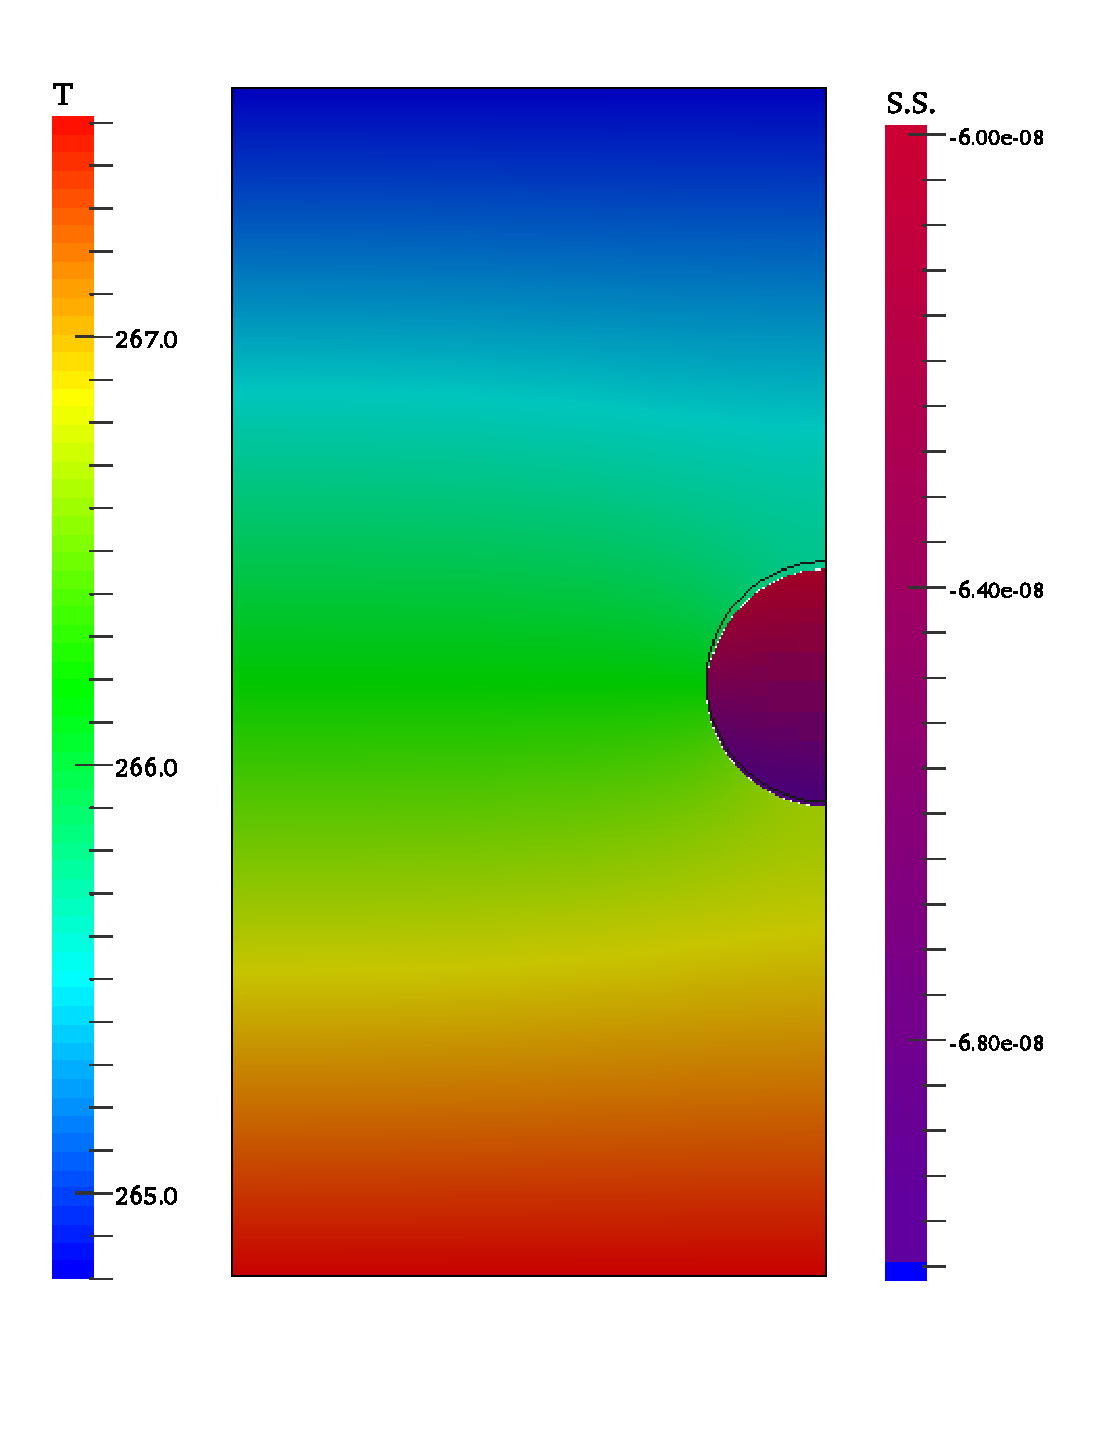
\includegraphics[width=\linewidth]{figures/bubble.pdf}
  \caption{Benchmark problem of bubble within \unit[5]{mm} cross section of ice; temperature (T) reported in \unit[]{K} and supersaturation (S.S.) in \unitfrac[]{kg}{m$^3$}.}
  \label{fig:bubble}
\end{figure}

Utilizing the simulation settings similar to the benchmark problem a simulation was performed on a $\mu$-CT scanned cross-section of snow measuring \unit[5]{mm} square. This sample was subjected to a temperature gradient of \unitfrac[250]{K}{m} for approximately eight hours.

As shown if Fig. \ref{fig:keff}, during the simulation the effective thermal conductivity ($k_{eff}$) was computed in the vertical (y) and horizontal directions (x), which were on the order of \unitfrac[1.2]{W}{mK}, which is on the upper limit of what is expected for snow \citep{sturm1997thermal}.

\begin{figure}
  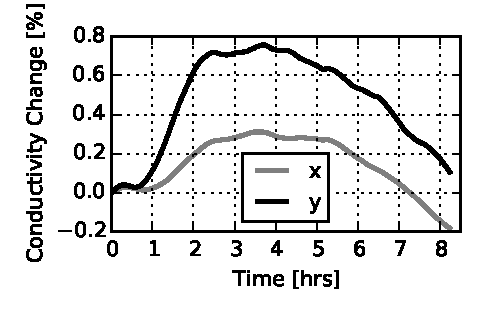
\includegraphics[width=\linewidth]{figures/pika_keff.pdf}
  \caption{Percent change in effective thermal conductivity in the vertical (y) and horizontal directions (x) during the simulations.}
  \label{fig:keff}
\end{figure}


Fig. \ref{fig:snow2d:diff} includes the raw snow image overlaid with the areas that observed sublimation (hot colors) and deposition (cold colors) and Fig. \ref{fig:snow2d:grains} snow the temperature field at the end of the simulation as well as the ice grain locations at the beginning and end of the simulations.

The $k_{eff}$ results are of particular interest, during the first few hours of the simulation both values increase, with the vertical direction increase at a greater rate. Then both begin to decrease at a similar rate after about four hours. There may be man explanations for this behavior, but considering the simplicity of the phae-change kinetics in the model such analysis is beyond the scope of this paper.

The results presented here serve as demonstration of the capabilities and potential to model micro-structure evolution of snow using MOOSE. Pika is intended as a starting point for further research that includes convection in the pore space, more realistic vapor flux boundary conditions, and enhanced phase-change kinetics including accounting for ice grain orientation.


\setlength{\unitlength}{1in}
\begin{figure}
  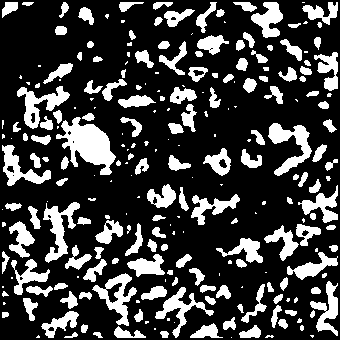
\includegraphics[width=\linewidth]{figures/snow2d_raw.png}
  \put(-3.125 ,0){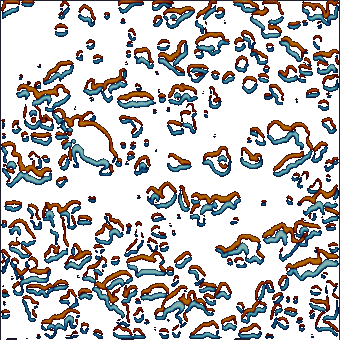
\includegraphics[width=\linewidth]{figures/diff_overlay.png}}
  \caption{The difference between the phase-field variable between initial and final simulations steps demonstrating where mass was gained (blue) and lost (orange).}
  \label{fig:snow2d:diff}
\end{figure}

\begin{figure}
  \includegraphics[width=\linewidth]{figures/snow2d_temp.pdf}
  \caption{The difference in the ice grains initially (black) and after (white) 8 hours subjected to a \unitfrac[250]{K}{m} temperature gradient.}
  \label{fig:snow2d:grains}
\end{figure}

\section{IBEX: MESO-SCALE MODEL}\label{sec:ibex}
The meso-scale model presented here is comprised of a single relationship, the heat-equation:3

\begin{equation}\label{eq:meso}
\rho c_p \frac{\partial{T}}{\partial t} = \nabla \cdot k_{eff} \nabla T + s,
\end{equation}
where $T$ is temperature, $s$ a heat source term, and the material properties $\rho$, $c_p$, and $k_{eff}$ are the bulk density, specific heat, and thermal conductivity for snow. The model developed includes incoming shortwave radiation that is absorbed within the snow (i.e., the $s$ source term in Eq. \eqref{eq:meso}), including absorption that differs with wavelength as detailed by \citet[][Ch. 4]{slaughter2010numerical}. On the surface the effects of incoming and out going long-wave radiation as well as sensible and latent heat are included as detailed in \citet{morstad2007experimental}.

To demonstrate the accuracy of the model, Exp. \#2 of \citet{morstad2007experimental} was reproduced using a 1D Ibex simulation. The simulation was similar fashion as detailed in \citet[][Ch. 4]{slaughter2010numerical}. For the simulation, all input parameters were set to the value discussed in detail in \citet{slaughter2010numerical}, including incoming short- and long-wave radiation set to \unitfrac[650]{W}{m\textsuperscript{2}} and \unitfrac[235]{W}{m\textsuperscript{2}}, respectively and the albedo in the visible, near-infrared, and short-wave infrared defined as 0.94, 0.80, and 0.59, respectively.

Fig. \ref{fig:ibex_1d} includes the simulation results and a comparison with the experimental data of \citet{morstad2007experimental} after 8 hours; qualitatively the 1D Ibex model is capable capturing the general trend of experimental data. Fine tuning the parameters for Ibex is beyond the scope of this paper.

\begin{figure}[h]
  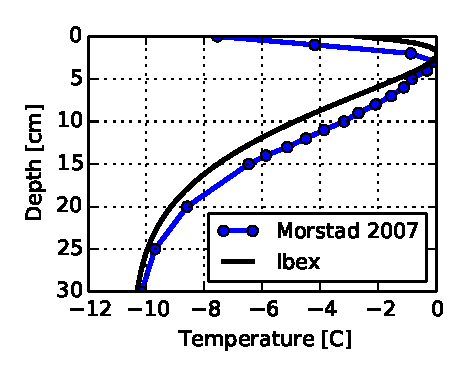
\includegraphics[width=3.125in]{figures/ibex.pdf}
  \caption{Comparison of experimental data and 1D Ibex simulation.}
  \label{fig:ibex_1d}
\end{figure}

Since, Ibex was built using MOOSE, it is dimension agnostic, thus the same code that produced the 1D results above is also capable of running in 3D with adaptive meshing, as shown in Fig. \ref{fig:ibex_3d}, without altering anything except the input file. This simulation uses the same input parameters as mentioned above, except applies the incoming short-wave irradiance as function of space and time. This demonstrates the flexibility of MOOSE-based application to build flexible and extensible applications, which will be further demonstrated in the next section.

\begin{figure}
  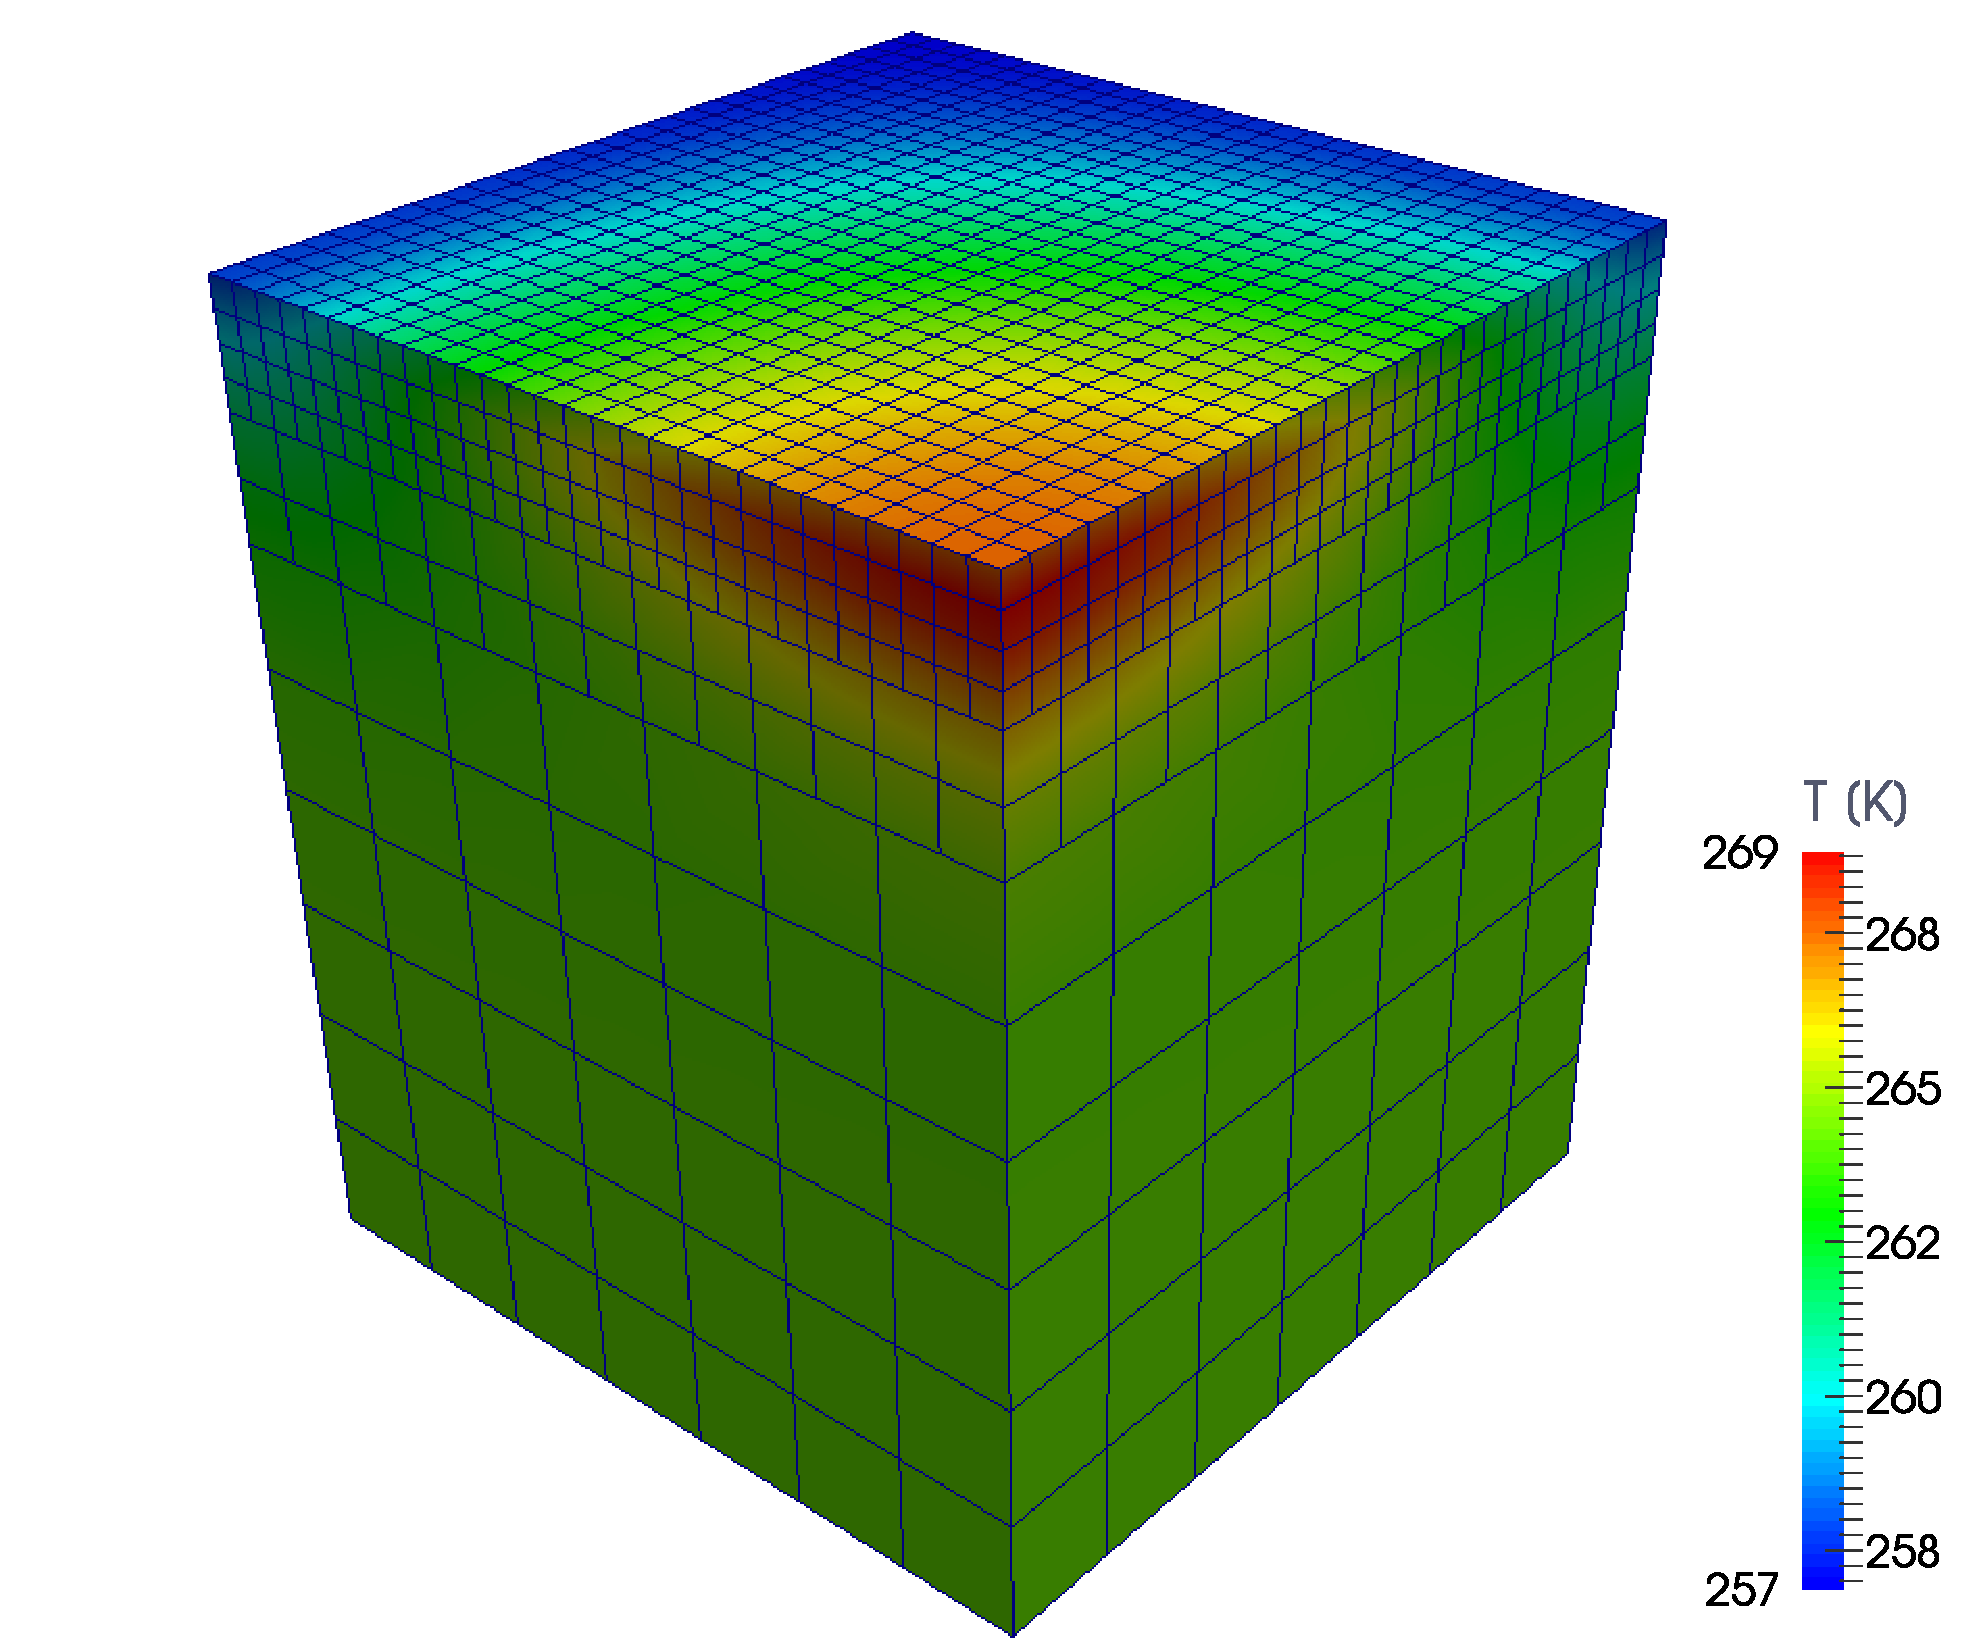
\includegraphics[width=\linewidth]{figures/ibex3d.pdf}
  \caption{Demonstration of 3D Ibex simulation with spatial and temporal varying incoming short-wave irradiance.}
  \label{fig:ibex_3d}
\end{figure}


\section{MULTI-SCALE MODEL}\label{sec:yeti}
add ref to MOOSE nuclear paper

\section{CLOSING REMARKS}
